\documentclass[fleqn]{article}
\oddsidemargin 0.0in
\textwidth 6.0in
\thispagestyle{empty}
\usepackage{import}
\usepackage{amsmath}
\usepackage{graphicx}
\usepackage{flexisym}
\usepackage{calligra}
\usepackage{amssymb}
\usepackage{bigints} 
\usepackage[english]{babel}
\usepackage[utf8x]{inputenc}
\usepackage{float}
\usepackage[colorinlistoftodos]{todonotes}


\DeclareMathAlphabet{\mathcalligra}{T1}{calligra}{m}{n}
\DeclareFontShape{T1}{calligra}{m}{n}{<->s*[2.2]callig15}{}
\newcommand{\scriptr}{\mathcalligra{r}\,}
\newcommand{\boldscriptr}{\pmb{\mathcalligra{r}}\,}

\definecolor{hwColor}{HTML}{442020}

\begin{document}

  \begin{titlepage}

    \newcommand{\HRule}{\rule{\linewidth}{0.5mm}}

    \center

    \begin{center}
      
\includegraphics[height=11cm, width=11cm]{asu.png}
    \end{center}

    \vline

    \textsc{\LARGE Statistical/Thermal Physics}\\[1.5cm]

    \HRule \\[0.5cm]
    { \huge \bfseries Homework 9}\\[0.4cm] 
    \HRule \\[1.0cm]

    \textbf{Behnam Amiri}

    \bigbreak

    \textbf{Prof: Michael Treacy}

    \bigbreak

    \textbf{{\large \today}\\[2cm]}

    \vfill

  \end{titlepage}

  \begin{enumerate}
    \item \textbf{5.16} A formula analogous to that for $C_P-C_V$ relates the isothermal and 
    isentropic compressibilities of a material:
    $$
      \kappa_T=\kappa_S+\dfrac{TC \beta^2}{C_P}
    $$
    (Here $\kappa_S=-\dfrac{1}{V} \bigg( \dfrac{\partial V}{\partial P} \bigg)_S $) is the...

    \begin{center}
      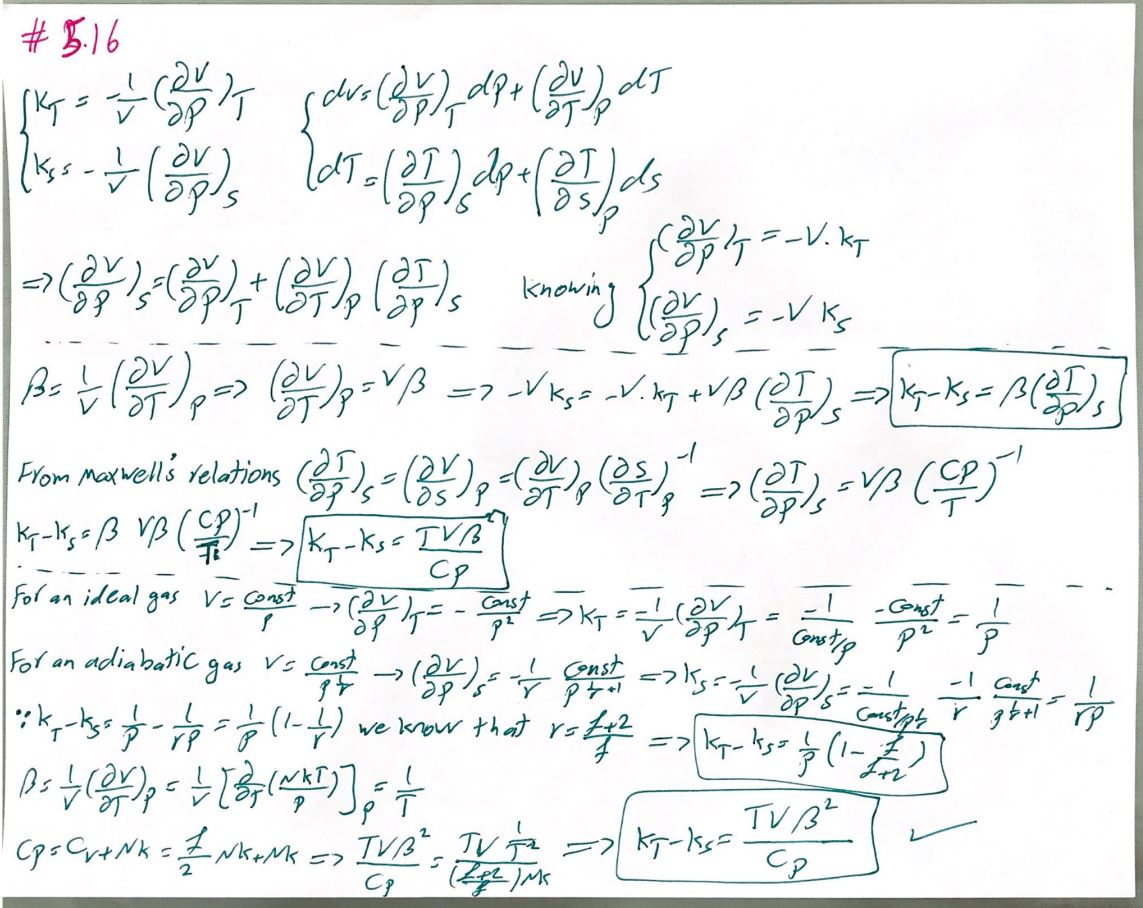
\includegraphics[height=16cm, width=17cm]{516.JPG}
    \end{center}

    \pagebreak

    \item \textbf{5.20} The first excited energt level of a hydrogen atom has an energy of $10.2 ~ eV$, if
    we take the ground-state energy to be zero...

    \begin{center}
      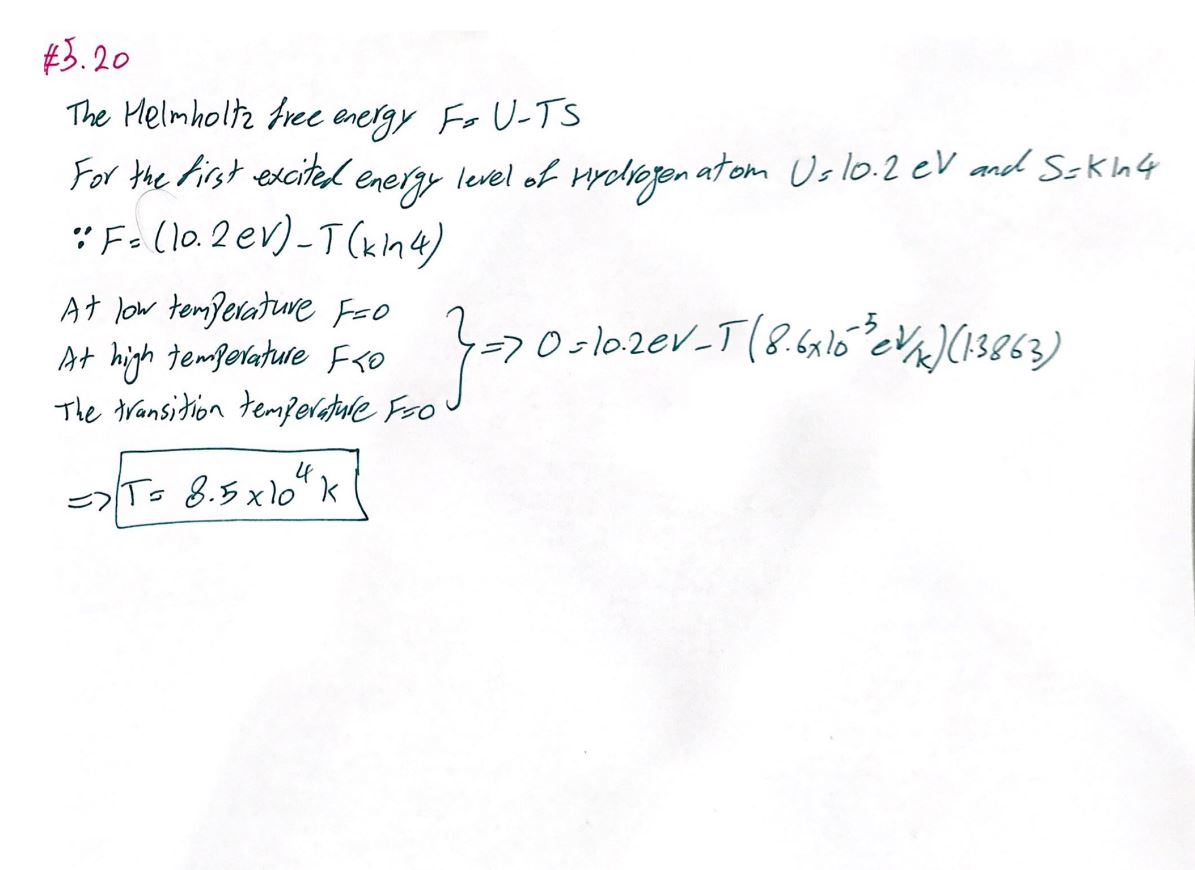
\includegraphics[height=16cm, width=17cm]{520.JPG}
    \end{center}
    \pagebreak

    \item \textbf{5.21} Is heat capacity ($C$) extensive or intensive? What about specific heat ($c$)?
    Explain briefly.

    \begin{center}
      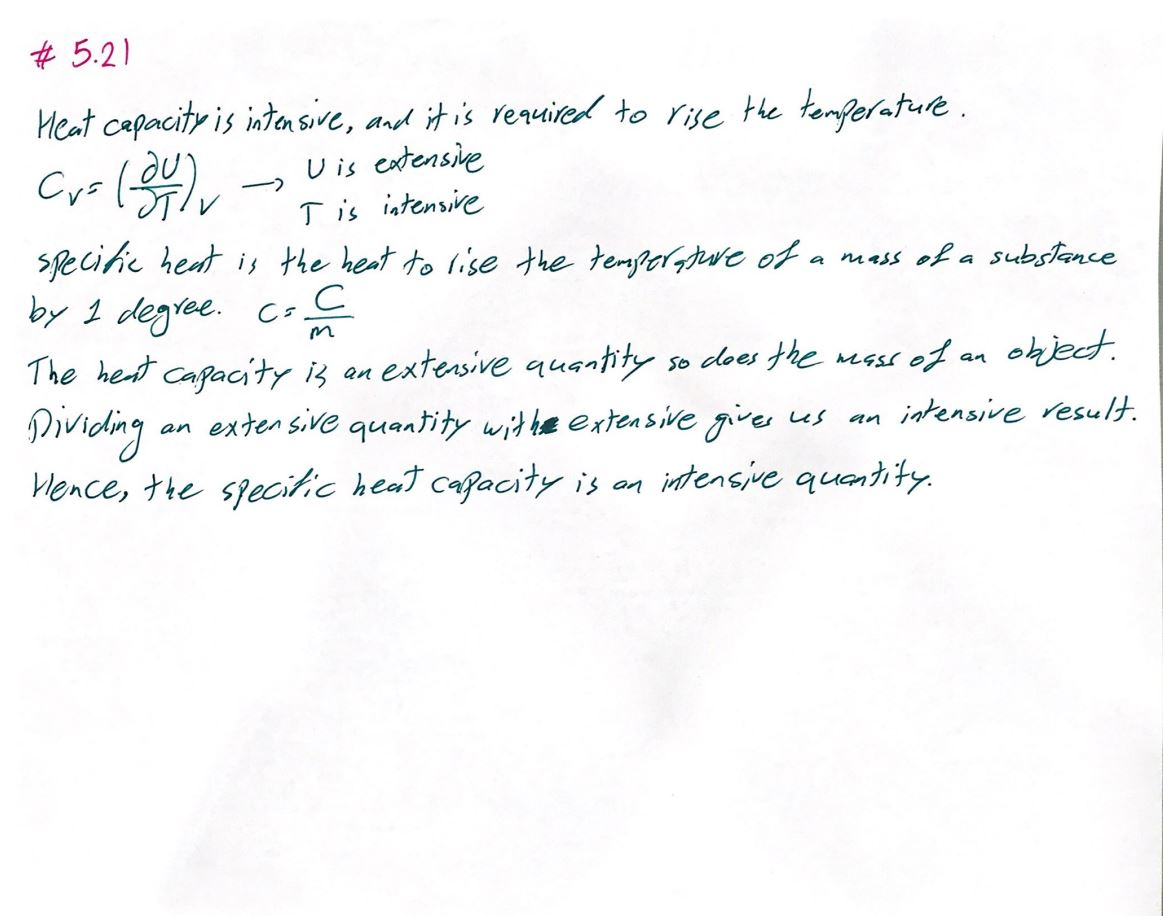
\includegraphics[height=16cm, width=17cm]{521.JPG}
    \end{center}
    \pagebreak

    \item \textbf{5.23} (use eqn. (3.63) for the chemical potential) By subtracting $\mu U$ from 
    $U, H, F,$ or $G$, one can obtain four new thermodynamics potentials. Of the four, the most useful
    is the \textbf{grand free energy} (or \textbf{grand potential}),
    $$
      \Phi=U-TS-\mu N.
    $$
    \begin{enumerate}
      \item Derive the thermodynamic identity for $\Phi$, and...

      \item Prove that, for a system in thermal and diffusive equilibrium...

      \item Prove that $\Phi=-PV$.

      \item As a simple application, let the system be a single proton, which can be "occupied"
      either by a single electron...
    \end{enumerate}

    \begin{center}
      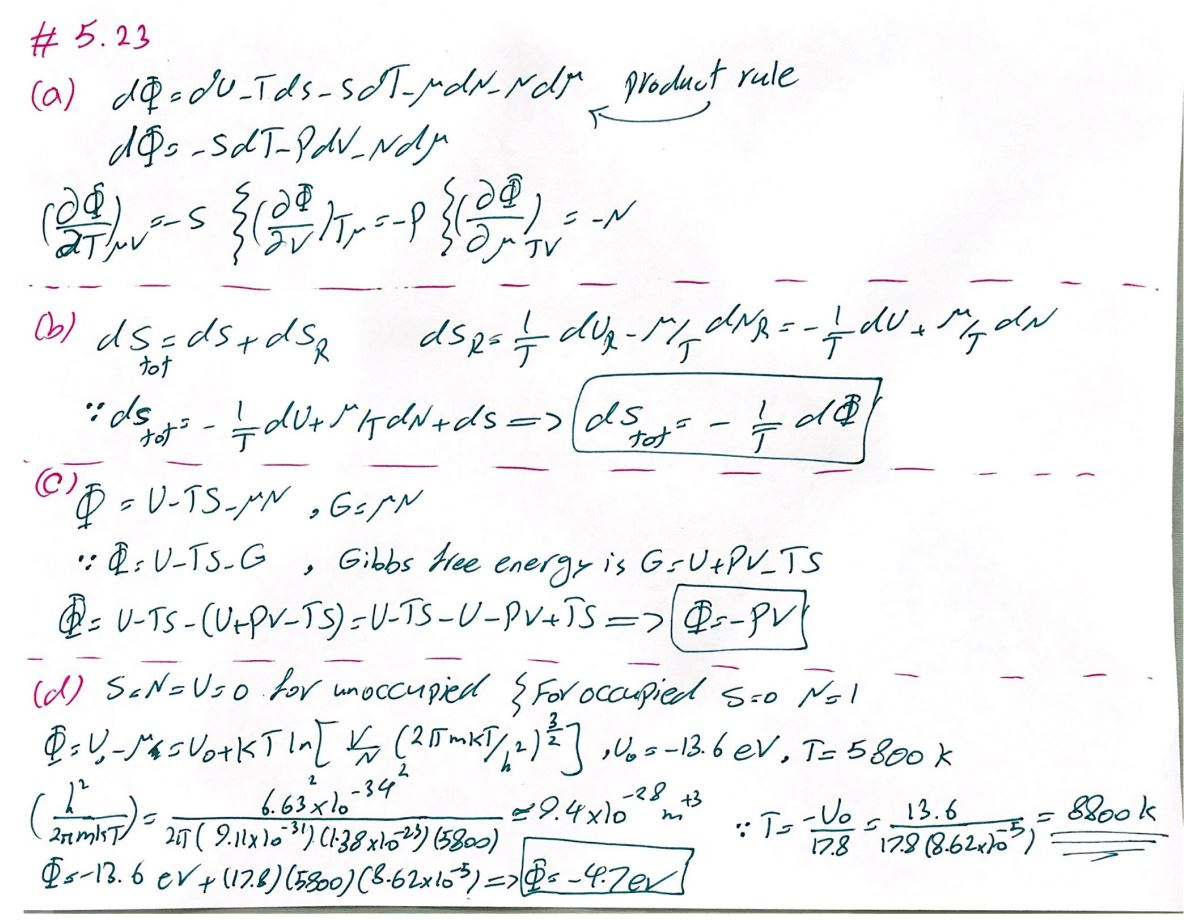
\includegraphics[height=14cm, width=17cm]{523.JPG}
    \end{center}

    \pagebreak

    \item \textbf{5.27} Graphite is more compressible than diamond.
    \begin{enumerate}
      \item Taking compressibilities into account, would you expect...

      \item The isothermal compressibility of graphite is about $3 \times 10^{-6} ~ bar^{-1}$, 
      while that of diamond is more than ten times less...

    \end{enumerate}

    \begin{center}
      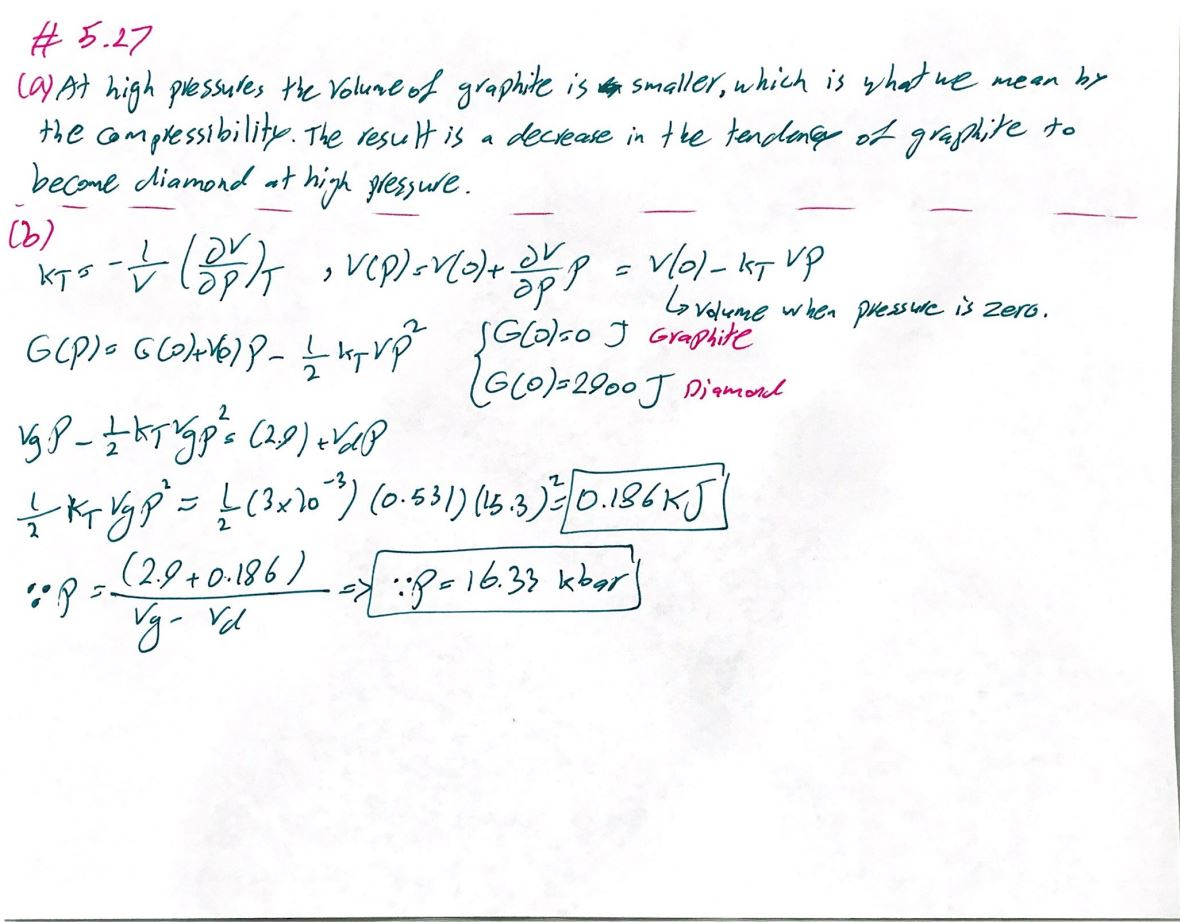
\includegraphics[height=16cm, width=17cm]{527.JPG}
    \end{center}

    \pagebreak

    \item \textbf{5.32} The density of ice is $917 ~ kg/m^3$.
    \begin{enumerate}
      \item Use the Clausius-Clapeyron relation to explain why the slope...

      \item How much pressure would you have to put...

      \item Approximately how deep under a glacier would you have to be before the 
      weight of the ice above gives the pressure you found in part (b)?...

      \item Make a rough estimate of the pressure under the blade of an ice skate, and 
      calculate the melting temperature of ice at this pressure...

    \end{enumerate}

    \begin{center}
      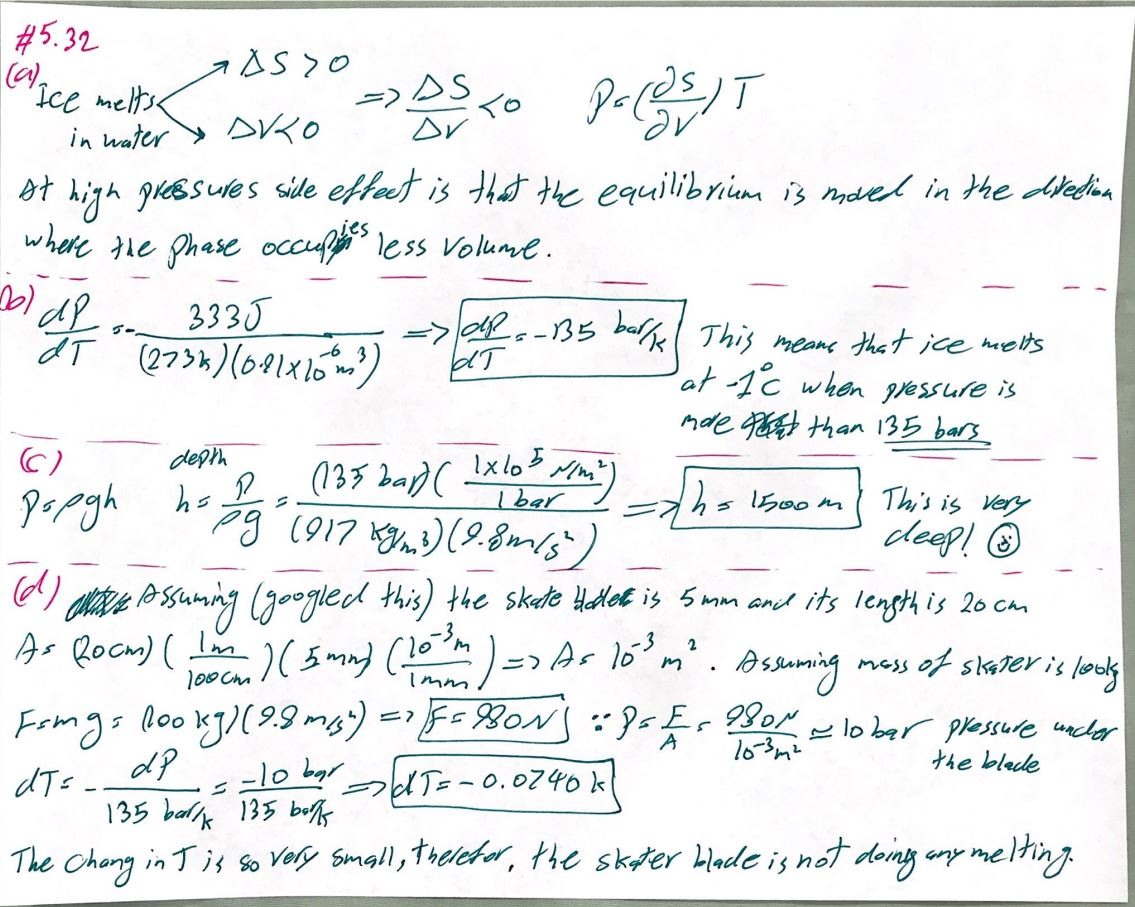
\includegraphics[height=14cm, width=17cm]{532.JPG}
    \end{center}


  \end{enumerate}

\end{document}
